% Chapters
\chapter{Sprint Planning}\label{chap:s4_sprintplanning}

\begin{chapterorganization}
  \item in \sectionref{sec:S4_bd} we describe the user stories we commit ourselves to during the \bd sprint planning meeting.
  \item in \sectionref{sec:S4_group} we describe the sprint planning in our group and lists our tasks with reference to a user story.
\end{chapterorganization}

\section{\bdtitle Sprint Planning}\label{sec:S4_bd}
During the \bd sprint planning we choose to work on the following user stories in this sprint. They are labeled with a number in parentheses for reference.

\todo{Tilføj conditions of satisfaction}

\begin{description}
  \item[Job Prioritization on Jenkins (1)] Developers have specified a desire for some jobs to have a higher priority than other jobs. For example developers would like libraries to run before apps.
  \item[Monkey Test on Debug Versions of Apps (2)] With the \db groups working on implementing database sync, they are making a test database available. Monkey tests currently use a development database that might be wiped accidentally. To ensure this does not happen monkey tests should run on debug APKs rather than release APKs.
  \item[Decrease Build Times on Jenkins Further (3)] When the queue on Jenkins is long, jobs can take a very long time to build. As we discussed in \sectionref{sec:non-emulator_testing}, the build times can be further reduces by working on the emulator.
  \item[Easy Download and Installation of all Apps (4)] In the previous sprint developers were not always using the latest versions of all apps, which lead to issues at the sprint end. The developers therefore want an easy way to download and install the newest version of all apps on their devices.
  \item[Document Jenkins Structure for Next Semester (5)] To make it easy for the next semester to start working with Jenkins, documentation of the Jenkins structure used is needed.
\end{description}

\section{Group Sprint Planning}\label{sec:S4_group}
At our internal sprint planning we divide the chosen user stories into tasks and estimate them. For this sprint, we have a total of 70 half days of work. \tableref{tab:sprint4_tasks} shows the tasks we have committed to solve for this sprint. Tasks with a plus (+) are tasks that have been added during the sprint as they were discovered.

\begin{table}%
  \centering
  \begin{tabular}{p{0.6\textwidth}rr}
    \toprule
    \textbf{Task} & \textbf{User Story} & \textbf{Estimation} \\
    \midrule
    Investigate conditions of satisfaction for our user stories & na & 2 \\
    Make a program to download and install the newest version of each app & 4 & 2 \\
    Make it so that the Android emulator is only started when no other devices are connected & 3 & 6 \\
    Connect to all Android devices wirelessly & 3 & 2 \\
    Connect Android devices permanently to the Internet & 3 & 2 \\
    Put debug APKs onto the ftp & 2 & 1 \\
    Make monkey tests use debug APKs & 2 & 1 \\
    Install Jenkins Prioritization Plugin & 1 & 1 \\
    Choose schedule for prioritization plugin & 1 & 2 \\
    Identify areas for Jenkins documentation (spike) & 5 & 2 \\
    Write about Jenkins files on server (from spike) & 5 & 2 \\
    Write about Jenkins structure (from spike) & 5 & 2 \\
    Investigate method to decrease emulator usage time (spike) & 3 & 1 \\
    % \midrule
    % \textbf{Down-prioritized tasks} & & \\
    % \midrule
    % \midrule
    % \textbf{Missed tasks} & & \\
    % \midrule
    % \textbf{Rejected tasks} & & \\
    % \midrule
    \midrule
    \textbf{Original total} & & y \\
    \textbf{Total} & & x \\
    \bottomrule
  \end{tabular}
\caption[Sprint 4 backlog]{Sprint backlog for sprint 4, excluding report tasks. The tasks are listed in no particular order.}
\label{tab:sprint4_tasks}
\end{table}

\todo{Tasken ``Investigate method to decrease emulator usage time (spike)''har vi ikke, men lavede uformelt den første dag da vi lavede sprint planning i gruppen}

\todo{I dette sprint skal vi også skrive frontmatter, backmatter, introduktion og konklusion}

\chapter{Upload of Apps to google play}
One of the user stories selected in this sprint is ``Automatic upload of alpha releases to google play´´. Currently the Jenkins server compiles the code but does nothing with the APKs. Before the APKs can be publish on Google Play, they need to be signed with our signature. The android plug-in for Gradle has functionality for automatic signing of APKs. We use this to sign. To sign we need a keystore file. We are not interested in everybody having this file as it serves as a proof of identification. We save the file on the server, which means that it becomes impossible to build a release version of the apps locally.
Every app has a version code, which is incremented every time a new release is published. This is not done per default, sp we need to set up the build to increase the version code every time a app is successfully built. 
Now the apks have been signed, we need to upload them. This can be done in two ways: via Jenkins \parencite{jenkins-play-plugin} or through Gradle \parencite{gradle-play-plugin}. The Jenkins plugin is easy to use, but requires that you know the exact name and location of the of the apk to upload.


\chapter{Some Chapter}
\section{Improving Build Times}

To identify in which parts of the build process to make faster, we measure the time different parts of the Launcher project take. The Launcher project is the main application which depends on many other subprojects. The timings are measured on the Jenkins server and shown in \figureref{fig:launcher_build_times}. The shows the build timings of the Launcher application and the different subprojects (\emph{Oasis-lib, Giraf-Component, Local-db, Barcode-scanner, and Metadata}), as well as the startup time for the emulator.\todo{Kan vi regne med, at submoduler bliver binære filer?}

\begin{figure}
\centering
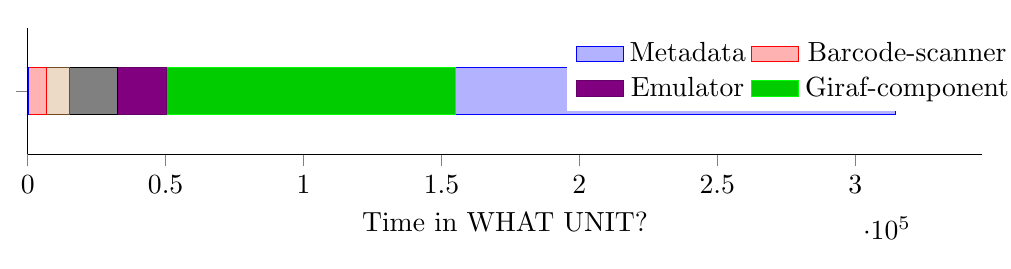
\begin{tikzpicture}[trim axis left, trim axis right]
  \begin{axis}[
    xbar stacked,
    scale only axis,
    width=\textwidth,
    axis y line*= none, axis x line*= bottom,
    %xmajorgrids = true,
    ytick = data,
    yticklabels = {},
    tick align = outside,
    %xtick pos = left,
    bar width=6mm,
    y=8mm,
    %nodes near coords,
    legend style={
      legend columns=4,
      anchor=north,
      yshift=0ex,
      xshift=0ex,
      draw=none
      %legend cell align=left
    },
    area legend,
    xlabel = {Time in WHAT UNIT?},
    xmin = 0
  ]
    \addplot coordinates
    {(209,0)}; 
    \addlegendentry{Metadata}
    \addplot coordinates
    {(6625,0)};
    \addlegendentry{Barcode-scanner}
    \addplot coordinates
    {(8393,0)};
    \addlegendentry{Launcher}
    \addplot coordinates
    {(17223,0)};
    \addlegendentry{Local-db}
    \addplot coordinates
    {(18000,0)};
    \addlegendentry{Emulator}
    \addplot coordinates
    {(104696,0)};
    \addlegendentry{Giraf-component}
    \addplot coordinates
    {(159497,0)};
    \addlegendentry{Oasis-lib}
    %\legend{Test, test, test, test, test, test}
  \end{axis}
\end{tikzpicture}
\caption{Timings during build of the Launcher project.}\label{fig:launcher_build_times}
\end{figure}

\chapter{Sprint Review}\label{chap:sprint3_end}

\begin{chapterorganization}
  \item in \sectionref{sec:s2_goals} we evaluate how the sprint went and whether we reached our goals on a group level.
  \item in \sectionref{sec:s2_multiprj_review} we evaluate how the sprint went on the multi project level.
\end{chapterorganization}

\section{Sprint Goals}\label{sec:s3_goals}
\dummy

\section{Multi-Project Sprint Review}\label{sec:s3_multiprj_review}
\dummy
